\documentclass[12pt]{article}

\usepackage[utf8]{inputenc}
\usepackage[T1]{fontenc}
\usepackage[polish,provide=*]{babel}
\usepackage{lmodern}
\usepackage{amsmath}
\usepackage{latexsym,amsfonts,amssymb,amsthm,amsmath}
\usepackage{enumitem}
\usepackage{hyperref}
\usepackage{graphicx}
\usepackage{float}
\usepackage{subcaption}
\usepackage{booktabs}
\graphicspath{{./images/}}

\setlength{\parindent}{0in}
\setlength{\oddsidemargin}{0in}
\setlength{\textwidth}{6.5in}
\setlength{\textheight}{8.8in}
\setlength{\topmargin}{0in}
\setlength{\headheight}{18pt}

\title{Wyznaczanie ruchliwości i koncentracji nośników w półprzewodniku}
\author{Kacper Kłos}

\begin{document}

\maketitle
W niniejszym artykule wyznaczyliśmy podstawowe parametry próbki domieszkowanego germanu (Ge) o znanej geometrii. Najpierw, mierząc napięcie i natężenie prądu dostarczanego do próbki, dopasowaliśmy krzywą, która pozwoliła nam określić przewodność w warunkach pokojowych: $\sigma = 56{,}10 \pm 0{,}05 \,\Omega^{-1}\mathrm{m}^{-1}$. Następnie, na podstawie pomiarów przeprowadzonych przy różnych wartościach natężenia prądu oraz pola magnetycznego, wyznaczyliśmy stałą Halla $R_h = (5{,}30 \pm 0{,}03)\times 10^{-3} \,\mathrm{m}^3\mathrm{C}^{-1}$. Analizując znaki uzyskanego napięcia Halla w pojedynczych pomiarach, stwierdziliśmy, że dominującymi nośnikami ładunku w próbce są nośniki dodatnie. Łącząc wszystkie wcześniejsze wyniki, obliczyliśmy ruchliwość nośników $\mu = 2922 \pm 4 \,\mathrm{cm}^2\mathrm{s}^{-1}\mathrm{V}^{-1}$ oraz ich koncentrację, wynoszącą $(1{,}1985 \pm 0{,}0013) \times 10^{15} \,\mathrm{cm}^{-3}$ (obydwie wielkości w temperaturze pokojowej). Na koniec sprawdziliśmy wpływ wzrostu temperatury na koncentrację oraz ruchliwość nośników i wyznaczyliśmy energię aktywacji domieszek. Zauważyliśmy, że w miarę podnoszenia temperatury mobilność nośników maleje, podczas gdy ich koncentracja rośnie. Dopasowując otrzymane zależności do modelu teoretycznego, oszacowaliśmy energię aktywacji nośników samoistnych na $E_{A_s} = 0{,}658 \pm 0{,}018 \,\mathrm{eV}$.

\newpage
\section{Wstęp}
W niniejszym doświadczeniu przeprowadzamy analizę domieszkowanej próbki Ge za pomocą amperomierza, woltomierzy, grzałki, cewek oraz magnetometru. Naszym celem jest wyznaczenie przewodności próbki w temperaturze pokojowej, a także stałej Halla. Na podstawie tych wielkości obliczamy koncentrację nośników, ich ruchliwość oraz znak nośników. Na koniec badamy, jak zachowują się koncentracja i ruchliwość w zależności od temperatury, a następnie dopasowujemy krzywą do obserwowanej zależności, co pozwala nam wyznaczyć energię aktywacji domieszek.

\section{Podstawy Teoretyczne}
Przedstawione niżej wyprowadzenia wzorów wykorzystanych w doświadczeniu stanowią skrótowe omówienie wyprowadzeń zawartych w~\cite{skrypt}.

Gdy do próbki nie jest przyłożone żadne napięcie, nośniki ładunku poruszają się w sposób losowy. Po przyłożeniu wyższego potencjału na jednym końcu próbki wytwarza się pole elektryczne, które nadaje nośnikom składową prędkości zależną od ich znaku. Całość można opisać wzorem:
\begin{equation}
    \sigma = |q|\,n\,\mu,
    \label{eq:conductivity}
\end{equation}
gdzie $\sigma$ to przewodność, $q$ jest ładunkiem nośnika, $n$ to koncentracja nośników (liczba nośników w jednostce objętości), a $\mu$ oznacza mobilność (ruchliwość).

Możemy też rozpisać prawo Ohma: $U = R\,I$, przy czym rezystancję $R$ wyrażamy przez przewodność oraz geometrię próbki:
\begin{equation}
    U = \frac{1}{\sigma}\,\frac{l}{S}\, I,
    \label{eq:ohm_law}
\end{equation}
gdzie $l$ to długość próbki, $S$ jest jej polem przekroju, a $I$ oznacza natężenie prądu. Wzór ten pozwala wyznaczyć $\sigma$ na podstawie wielkości mierzalnych.

\begin{figure}[H]
    \centering
    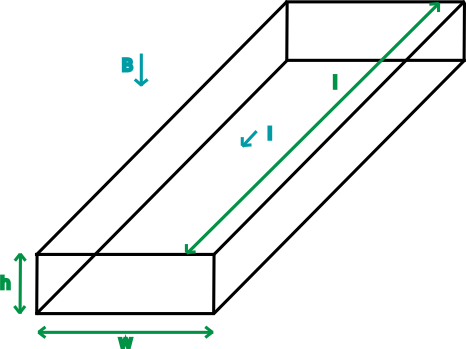
\includegraphics[scale=1.3]{probka}
    \caption{Geometria badanej próbki}
    \label{fig:probka}
\end{figure}

Efekt Halla przejawia się w obecności pola magnetycznego $B$: na nośniki działa siła Lorentza $F_M = q\,(\vec{v} \times \vec{B})$ oraz siła elektryczna wywołana rozdzieleniem ładunków, $F_E = U_H\,w$ w przypadku geometrii z rys.~\ref{fig:probka}, gdzie $U_H$ to napięcie Halla, a $w$ jest wymiarem próbki w poprzek prądu i pola. Po osiągnięciu równowagi sił i uwzględnieniu związku między prędkością nośników a prądem w próbce, otrzymujemy:
\begin{equation}
    U_H = \frac{1}{n\,q}\,\frac{I\,B}{h},
    \label{eq:hall_voltage}
\end{equation}
gdzie $h$ to grubość próbki w kierunku prostopadłym do wektora prądu i pola magnetycznego. Współczynnik $R_H = \tfrac{1}{n\,q}$ nazywamy stałą Halla. Znak napięcia Halla pozwala ustalić, czy nośniki są dodatnie (dziury), czy ujemne (elektrony).

Dla półprzewodników domieszkowanych wyróżnia się trzy główne zakresy temperatur (niski, średni i wysoki) z charakterystycznymi zależnościami przewodności $\sigma$ od $T$, przy czym w zakresie wyższych temperatur (powyżej ok. $400\,\mathrm{K}$) zwykle spełniony jest wzór:
\begin{equation}
    \sigma = \sigma_0 \exp\!\biggl(-\frac{E_{A_s}}{2kT}\biggr),
    \label{eq:high_temp}
\end{equation}
gdzie $E_{A_s}$ jest energią aktywacji nośników samoistnych, a $k$ oznacza stałą Boltzmanna.

\section{Układ Doświadczalny}
Na rys.~\ref{fig:diagram} przedstawiamy schemat układu elektrycznego używanego w doświadczeniu. Napięcia $V_1$, $V_2$ i $V_3$ sterujemy za pomocą generatora DP832, co pozwala na płynne zwiększanie natężenia prądu w elektromagnesie (a tym samym pola magnetycznego) oraz napięcia na próbce. Dodatkowo korzystamy z magnetometru oraz kompasu, aby zidentyfikować wartość i kierunek pola w obszarze próbki.

\begin{figure}[H]
    \centering
    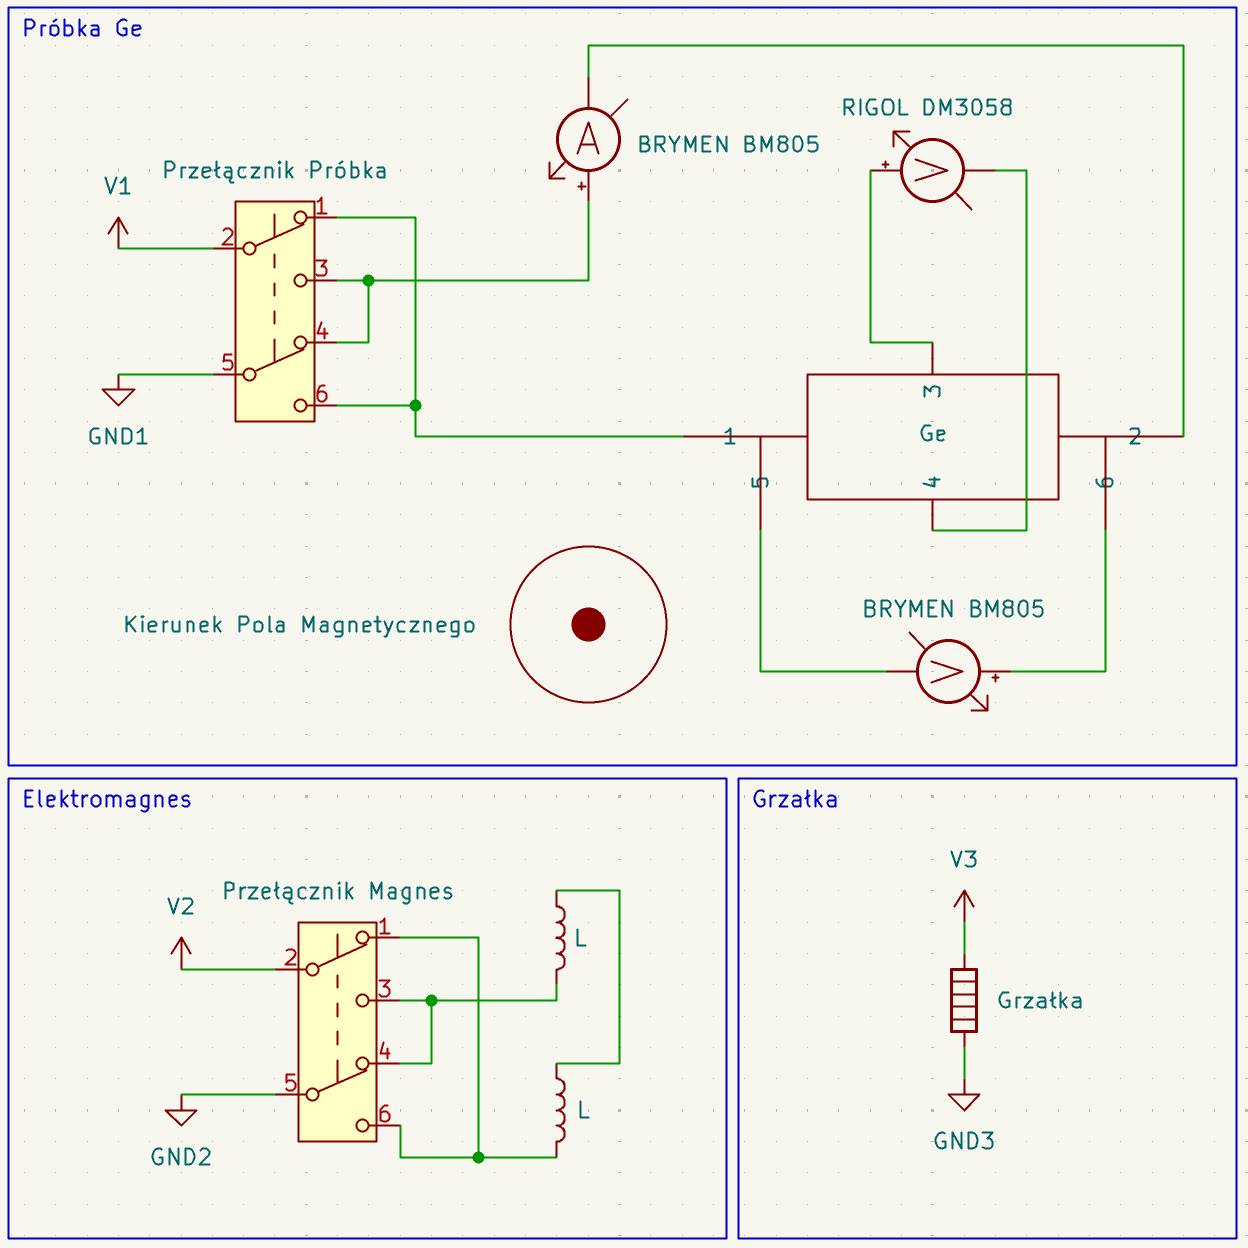
\includegraphics[scale=0.28]{diagram}
    \caption{Schemat układu pomiarowego (wykonany w \cite{diagram}).}
    \label{fig:diagram}
\end{figure}

Najpierw dopasowujemy prostą do zależności napięcia od natężenia na próbce, co pozwala określić jej przewodność. Następnie wykonujemy dwie serie pomiarów napięcia Halla: jedną przy stałym polu magnetycznym, a zmiennym natężeniu na próbce, a drugą przy stałym natężeniu i zmiennym polu. Aby wyeliminować zakłócenia od nierównomierności próbki, rejestrujemy napięcia Halla w czterech konfiguracjach (odwracając kierunek prądu oraz kierunek pola). Efektywne napięcie Halla wyznaczamy wzorem
\begin{equation}
    U_H = \frac{U_1 - U_2 + U_3 - U_4}{4},
    \label{eq:effective_hall}
\end{equation}
gdzie $U_1, U_2, U_3, U_4$ to odpowiednio napięcia mierzone w czterech konfiguracjach.

W ostatniej części doświadczenia ustalamy stałe napięcie na próbce i wybrane pole magnetyczne, po czym zmieniamy jej temperaturę (poprzez ogrzewanie i chłodzenie), rejestrując w każdym punkcie pomiarowym spadek napięcia na próbce, napięcie Halla oraz temperaturę.

\section{Wyniki Pomiarów}
Analizowana próbka ma geometrię analogiczną do rys.~\ref{fig:probka} o wymiary $20 \times 10 \times 1\,\mathrm{mm}^3$. W analizie błędów stosujemy notację $u(x)$ oznaczającą niepewność pomiarową wielkości $x$, a także wielokrotnie wykorzystujemy wzór na propagację błędu:
\[
    u\bigl(f(x_1,\dots,x_n)\bigr) \;=\; \sqrt{\sum_{i=1}^{n} \Bigl(\frac{\partial f}{\partial x_i}\,u(x_i)\Bigr)^2}.
\]

\subsection{Przewodność}
Badając zależność napięcia od natężenia dla różnych wartości dostarczanych przez zasilacz, przyjmujemy błędy pomiarowe multimetru \cite{multimeter_hand}: $u(U) = 0{,}5\%\text{ odczytu}$, $u(A) = 2\%\text{ odczytu}$.

\begin{table}[h]
    \centering
    \begin{tabular}{c|cc|cc}
        \toprule
        Nr & $I\,[\mathrm{mA}]$ & $u(I)\,[\mathrm{mA}]$ & $U\,[\mathrm{V}]$ & $u(U)\,[\mathrm{V}]$ \\
        \midrule
        1 & -26{,}82 & 0{,}14 & -0{,}96 & 0{,}02 \\
        2 & -20{,}08 & 0{,}10 & -0{,}714 & 0{,}015 \\
        3 & -24{,}74 & 0{,}13 & -0{,}882 & 0{,}018 \\
        4 & -19{,}73 & 0{,}10 & -0{,}704 & 0{,}014 \\
        5 & -9{,}69  & 0{,}05 & -0{,}345 & 0{,}007 \\
        6 & -4{,}70  & 0{,}03 & -0{,}167 & 0{,}004 \\
        \bottomrule
    \end{tabular}
    \caption{Pomiary napięcia na próbce przy różnych wartościach natężenia prądu.}
    \label{tab:ohm_measurements}
\end{table}

Na rys.~\ref{fig:ohm_measurments} przedstawiamy dopasowanie liniowe do punktów z tabeli \ref{tab:ohm_measurements}.  
\begin{figure}[H]
    \centering
    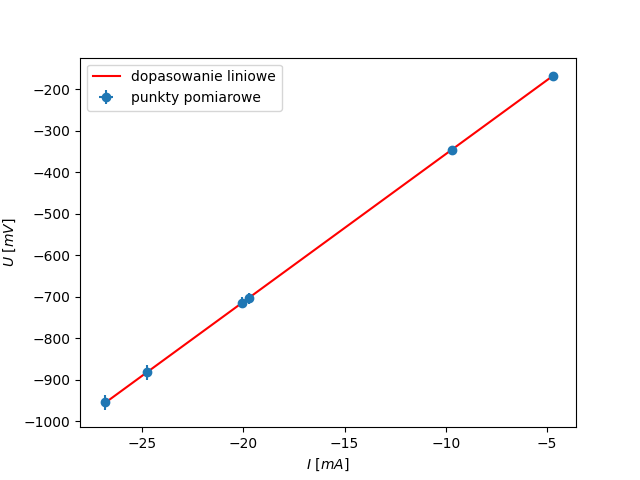
\includegraphics[scale=0.5]{ohm_law}
    \caption{Pomiary napięcia w funkcji natężenia (punkty) wraz z dopasowaną linią.}
    \label{fig:ohm_measurments}
\end{figure}

Z dopasowania uzyskaliśmy:
\begin{equation}
    R = 35{,}65\,\Omega, \quad u(R) = 0{,}04\,\Omega.
    \label{eq:resistance}
\end{equation}
Podstawiając do wzoru \ref{eq:ohm_law} wartość \eqref{eq:resistance} oraz wymiary próbki, otrzymujemy:
\begin{equation}
    \sigma = 56{,}10\,\Omega^{-1}\mathrm{m}^{-1}, \quad u(\sigma) = 0{,}05\,\Omega^{-1}\mathrm{m}^{-1}.
    \label{eq:final_conductivity}
\end{equation}
Niepewność $u(\sigma)$ wynika z propagacji błędu:
\[
    u(\sigma) \;=\; \biggl|\frac{l}{w\,h\,R^2}\biggr|\,u(R).
\]

\subsection{Stała Halla}
Dla analizy przyjmujemy \cite{magnetometer}: $u(B) = 5\%$, zaś błąd napięcia Halla \cite{multimeter_big} $u(U_H) = 0{,}015\%\!+\!0{,}008\,\mathrm{mV}$.
We wszystkich poniższych pomiarach napięcia halla na próbce $U_1$, $U_2$, $U_3$, $U_4$ mierzone są kolejno w ustawieniu ($+I,+B$), ($+I,-B$), ($-I,+B$), ($-I,-B$), gdzie plus oznacza przepływ prądu tak jak na rys.~\ref{fig:diagram}, a minus przestawiony przełącznik.

\paragraph{Pomiar przy stałym natężeniu prądu.}
Najpierw ustalamy $I = -26{,}8\,\mathrm{mA}$ (z niepewnością $u(I) = 0{,}6\,\mathrm{mA}$) i zmieniamy pole magnetyczne, co daje dane z tabeli \ref{tab:const_current_measurements}.

\begin{table}[H]
    \centering
    \begin{tabular}{c|ccc|ccccc}
        \toprule
        Nr & $B_{+}$ [mT] & $B_{-}$ [mT] & $u(B)$ [mT] & $U_1$ [mV] & $U_2$ [mV] & $U_3$ [mV] & $U_4$ [mV] & $u(U_H)$ [mV] \\
        \midrule
        1 & 53 & 57 & 3  & -7{,}44 & 8{,}13 & 7{,}43 & -8{,}15 & 0{,}01 \\
        2 & 46 & 50 & 3 & -6{,}457 & 7{,}123 & 6{,}454 & -7{,}145 & 0{,}009 \\
        3 & 39 & 43 & 3 & -5{,}430 & 6{,}159 & 5{,}424 & -6{,}148 & 0{,}009 \\
        4 & 32{,}5 & 35{,}3 & 1{,}8 & -4{,}625 & 5{,}158 & 4{,}520 & -5{,}161 & 0{,}009 \\
        5 & 18{,}5 & 22{,}0 & 1{,}1   & -2{,}572 & 3{,}245 & 2{,}560 & -3{,}256 & 0{,}009 \\
        6 & 6{,}7  & 7{,}5  & 0{,}4 & -0{,}800 & 1{,}183 & 0{,}785 & -1{,}196 & 0{,}009 \\
        7 & 64 & 67 & 4  & -8{,}80 & 9{,}54 & 8{,}79 & -9{,}57 & 0{,}01 \\
        8 & 58 & 61 & 4 & -7{,}99 & 8{,}67 & 7{,}98 & -8{,}69 & 0{,}01 \\
        \bottomrule
    \end{tabular}
    \caption{Zależność napięcia Halla $U_i$ od pola magnetycznego $B$ wraz z błędami tych wartości, przy stałym natężeniu $|I|=26{,}8\,\mathrm{mA}$ dla różych konfiguracji kierunków natężenia i pola magnetycznego.}
    \label{tab:const_current_measurements}
\end{table}

Pole magnetyczne różni się nieco między pomiarami, dlatego za jego wartość przyjmujemy średnią z $B_{+}$ i $B_{-}$, a niepewność $u(B)$ przyjmujemy jako większą z dwóch błędów (lub równą maksymalnemu rozrzutowi). Napięcie Halla $U_H$ obliczamy na podstawie wzoru \eqref{eq:effective_hall}.  
Dopasowanie do wzoru \eqref{eq:hall_voltage} (rys.~\ref{fig:const_current_measuremnts}) daje:
\[
    \frac{|R_{H_C}|}{h} = 5{,}30\,\mathrm{m}^2\mathrm{C}^{-1}, \quad u\bigl(\tfrac{|R_{H_C}|}{h}\bigr) = 0{,}03\,\mathrm{m}^2\mathrm{C}^{-1}.
\]
Mnożąc przez grubość $h$, otrzymujemy
\begin{equation}
    |R_{H_C}| = (5{,}30 \pm 0{,}03)\times 10^{-3} \,\mathrm{m}^3\mathrm{C}^{-1}.
    \label{eq:hall_constant_current}
\end{equation}

\begin{figure}[H]
    \centering
    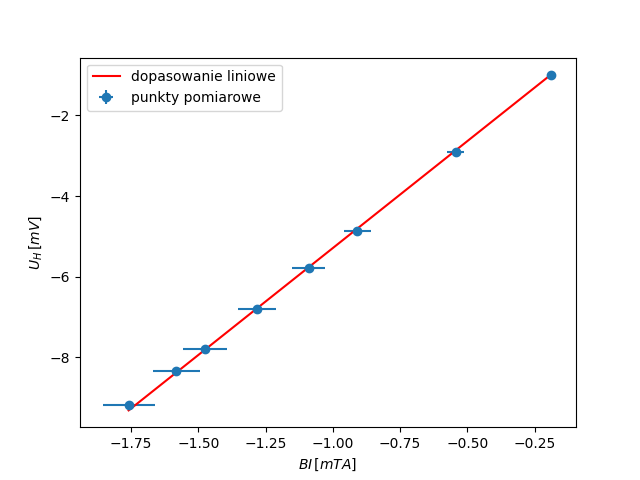
\includegraphics[scale=0.5]{const_current}
    \caption{Zależność napięcia Halla od iloczynu $B\,I$ przy stałym natężeniu (punkty pomiarowe z tabeli \ref{tab:const_current_measurements}) wraz z dopasowaniem.}
    \label{fig:const_current_measuremnts}
\end{figure}

\paragraph{Pomiar przy stałym polu magnetycznym.}
Analogicznie postępujemy przy pomiarach ze stałym polem (tabela \ref{tab:const_magnetic_field_measurements}), przyjmując $B \approx 66 \,\mathrm{mT}$ z niepewnością $u(B)=4\,\mathrm{mT}$.

\begin{table}[H]
    \centering
    \begin{tabular}{c|cc|ccccc}
        \toprule
        Nr & $I\,[\mathrm{mA}]$ & $u(I)\,[\mathrm{mA}]$ & $U_1\,[\mathrm{mV}]$ & $U_2\,[\mathrm{mV}]$ & $U_3\,[\mathrm{mV}]$ & $U_4\,[\mathrm{mV}]$ & $u(U_H)\,[\mathrm{mV}]$ \\
        \midrule
        1 & -26{,}8 & 0{,}6 & -8{,}82 & 9{,}55 & 8{,}80 & -9{,}56 & 0{,}01 \\
        2 & -21{,}7 & 0{,}5 & -7{,}13 & 7{,}72 & 7{,}14 & -7{,}74 & 0{,}01 \\
        3 & -16{,}8 & 0{,}4 & -5{,}517 & 5{,}952 & 5{,}512 & -5{,}963 & 0{,}009 \\
        4 & -11{,}8 & 0{,}3 & -3{,}882 & 4{,}188 & 3{,}881 & -4{,}192 & 0{,}009 \\
        5 & -6{,}82 & 0{,}14 & -2{,}247 & 2{,}419 & 2{,}242 & -2{,}426 & 0{,}009 \\
        6 & -28{,}9 & 0{,}6 & -9{,}53 & 10{,}28 & 9{,}51 & -10{,}29 & 0{,}01 \\
        7 & -2{,}70 & 0{,}06 & -0{,}898 & 0{,}968 & 0{,}899 & -0{,}972 & 0{,}009 \\
        \bottomrule
    \end{tabular}
    \caption{Zależność napięcia Halla $U_i$ od natężenia na próbce $I$ wraz z błędami tych wartości, przy stałym polu magnetycznym $|B|=66\,\mathrm{mT}$ dla różych konfiguracji kierunków natężenia i pola magnetycznego.}
    \label{tab:const_magnetic_field_measurements}
\end{table}

Dopasowanie do wzoru \ref{eq:hall_voltage} (rys.~\ref{fig:const_field_measuremnts}) daje:
\[
    \frac{|R_{H_B}|}{h} = 5{,}204\,\mathrm{m}^2\mathrm{C}^{-1}, \quad u\bigl(\tfrac{|R_{H_B}|}{h}\bigr) = 0{,}006\,\mathrm{m}^2\mathrm{C}^{-1},
\]
czyli
\begin{equation}
    |R_{H_B}| = (5{,}204 \pm 0{,}006)\times 10^{-3}\,\mathrm{m}^3\mathrm{C}^{-1}.
    \label{eq:hall_constant_field}
\end{equation}

\begin{figure}[H]
    \centering
    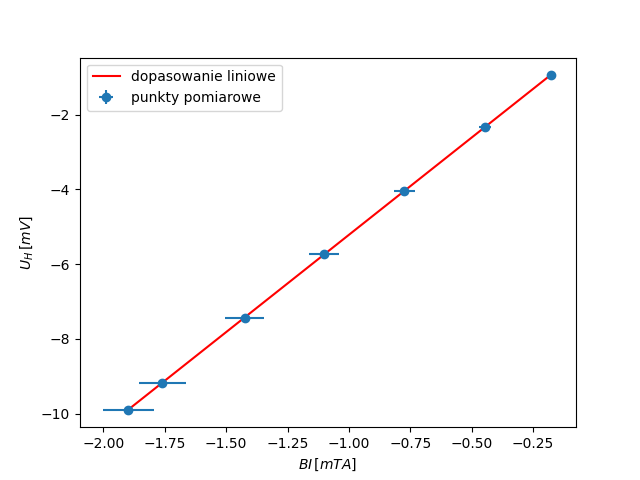
\includegraphics[scale=0.5]{const_field}
    \caption{Zależność napięcia Halla od iloczynu $B\,I$ przy stałym polu (punkty z tabeli \ref{tab:const_magnetic_field_measurements}) i dopasowana linia.}
    \label{fig:const_field_measuremnts}
\end{figure}

W celu uzyskania końcowej wartości $R_H$ stosujemy średnią ważoną z wartości \eqref{eq:hall_constant_current} i \eqref{eq:hall_constant_field}:
\[
    R_H = \frac{\frac{R_{H_C}}{u^2(R_{H_C})} + \frac{R_{H_B}}{u^2(R_{H_B})}}{\frac{1}{u^2(R_{H_C})} + \frac{1}{u^2(R_{H_B})}}, 
    \quad 
    u(R_H) = \frac{1}{\sqrt{\frac{1}{u^2(R_{H_C})} + \frac{1}{u^2(R_{H_B})}}}.
\]
Otrzymujemy:
\begin{equation}
    |R_H| = (5{,}208 \pm 0{,}006)\times 10^{-3}\,\mathrm{m}^3\mathrm{C}^{-1}.
    \label{eq:hall_const}
\end{equation}

\subsection{Znak nośników, ruchliwość i koncentracja ładunków}
Aby określić znak stałej Halla, przyglądamy się pomiarom napięć (z tabel \ref{tab:const_current_measurements} i \ref{tab:ohm_measurements}) oraz kierunkowi pola magnetycznego (ustalonemu za pomocą kompasu). Zauważyliśmy, że napięcia są ujemne w konfiguracji przyjętej na rys.~\ref{fig:diagram}, co sugeruje, iż głównymi nośnikami ładunku są dziury (dodatnie). Porównanie z orientacją pól $\vec{E}$ i $\vec{B}$ potwierdza, że stała Halla jest dodatnia:
\[
    R_H = +5{,}208 \times 10^{-3}\,\mathrm{m}^3\mathrm{C}^{-1}.
\]

Znając $R_H$ oraz przewodność $\sigma$, wyliczamy ruchliwość:
\[
    \mu = \sigma\,R_H, 
    \quad 
    u(\mu) = \sqrt{(\sigma\,u(R_H))^2 + (R_H\,u(\sigma))^2}.
\]
Podstawiając wartości z \eqref{eq:final_conductivity} i \eqref{eq:hall_const} otrzymujemy:
\begin{equation}
    \mu = 2922\,\mathrm{cm}^2\mathrm{s}^{-1}\mathrm{V}^{-1}, 
    \quad 
    u(\mu) = 4\,\mathrm{cm}^2\mathrm{s}^{-1}\mathrm{V}^{-1}.
    \label{eq:mobility}
\end{equation}

Korzystając z ładunku elementarnego \cite{charge} $q = 1{,}602\,176\,634 \times 10^{-19}\,\mathrm{C}$, możemy obliczyć koncentrację nośników:
\[
    n = \frac{1}{R_H\,q}, 
    \quad 
    u(n) = \frac{u(R_H)}{q\,R_H^2}.
\]
\begin{equation}
    n = (1{,}1985 \pm 0{,}0013)\times 10^{15}\,\mathrm{cm}^{-3}.
    \label{eq:density}
\end{equation}

\subsection{Zależność temperaturowa napięcia Halla}
W kolejnej części sprawdzamy, jak napięcie Halla na próbce zależy od temperatury. Ustawiamy stałe pole magnetyczne $B = 63{,}8 \pm 4\,\mathrm{mT}$ oraz natężenie prądu $I = -26{,}9 \pm 0{,}6\,\mathrm{mA}$. Temperaturę mierzymy termometrem z błędem $(0{,}1\% + 1\,^\circ\mathrm{C})$.

\begin{table}[H]
    \centering
    \begin{tabular}{c|cc|cc|cc}
        \toprule
        Nr & $T\,[^\circ \mathrm{C}]$ & $u(T)\,[^\circ \mathrm{C}]$ & $U_H\,[\mathrm{mV}]$ & $u(U_H)\,[\mathrm{mV}]$ & $U_P\,[\mathrm{V}]$ & $u(U_P)\,[\mathrm{V}]$ \\
        \midrule
        1  & 34{,}6  & 1 & -8{,}521 & 0{,}008 & -1{,}047 & 0{,}006 \\
        2  & 45{,}2  & 1 & -8{,}130 & 0{,}008 & -1{,}126 & 0{,}006 \\
        3  & 54{,}3  & 1 & -7{,}776 & 0{,}008 & -1{,}188 & 0{,}006 \\
        4  & 65{,}1  & 1 & -7{,}190 & 0{,}008 & -1{,}253 & 0{,}007 \\
        5  & 75{,}1  & 1 & -6{,}443 & 0{,}008 & -1{,}287 & 0{,}007 \\
        6  & 85{,}2  & 1 & -5{,}488 & 0{,}008 & -1{,}265 & 0{,}007 \\
        7  & 96{,}7  & 1 & -4{,}235 & 0{,}008 & -1{,}150 & 0{,}006 \\
        8  & 104{,}8 & 1 & -3{,}424 & 0{,}007 & -1{,}017 & 0{,}005 \\
        9  & 118{,}5 & 1 & -2{,}362 & 0{,}007 & -0{,}757 & 0{,}004 \\
        10 & 126{,}7 & 1 & -1{,}873 & 0{,}007 & -0{,}623 & 0{,}004 \\
        11 & 134{,}3 & 1 & -1{,}498 & 0{,}007 & -0{,}510 & 0{,}003 \\
        12 & 140{,}6 & 1 & -1{,}187 & 0{,}007 & -0{,}435 & 0{,}003 \\
        13 & 145{,}4 & 1 & -1{,}037 & 0{,}007 & -0{,}382 & 0{,}002 \\
        \bottomrule
    \end{tabular}
    \caption{Pomiary napięcia Halla $U_H$ i napięcia na próbce $U_P$ od tempertatury $T$ podczas ogrzewania wraz z błędami pomiarowymi.}
    \label{tab:heating_measurements}
\end{table}

\begin{table}[H]
    \centering
    \begin{tabular}{c|cc|cc|cc}
        \toprule
        Nr & $T\,[^\circ \mathrm{C}]$ & $u(T)\,[^\circ \mathrm{C}]$ & $U_H\,[\mathrm{mV}]$ & $u(U_H)\,[\mathrm{mV}]$ & $U_P\,[\mathrm{V}]$ & $u(U_P)\,[\mathrm{V}]$ \\
        \midrule
        1  & 143{,}8 & 1 & -1{,}117 & 0{,}007 & -0{,}410 & 0{,}002 \\
        2  & 136{,}2 & 1 & -1{,}402 & 0{,}007 & -0{,}506 & 0{,}003 \\
        3  & 127{,}3 & 1 & -1{,}773 & 0{,}007 & -0{,}627 & 0{,}004 \\
        4  & 120{,}3 & 1 & -2{,}183 & 0{,}007 & -0{,}742 & 0{,}004 \\
        5  & 112{,}1 & 1 & -2{,}800 & 0{,}007 & -0{,}891 & 0{,}005 \\
        6  & 105{,}3 & 1 & -3{,}408 & 0{,}008 & -1{,}018 & 0{,}005 \\
        7  & 97{,}5  & 1 & -4{,}201 & 0{,}008 & -1{,}147 & 0{,}006 \\
        8  & 86{,}6  & 1 & -5{,}452 & 0{,}008 & -1{,}258 & 0{,}007 \\
        9  & 75{,}3  & 1 & -6{,}505 & 0{,}008 & -1{,}281 & 0{,}007 \\
        10 & 66{,}2  & 1 & -7{,}219 & 0{,}008 & -1{,}255 & 0{,}007 \\
        11 & 55{,}5  & 1 & -7{,}825 & 0{,}008 & -1{,}159 & 0{,}006 \\
        12 & 44{,}2  & 1 & -8{,}267 & 0{,}008 & -1{,}112 & 0{,}006 \\
        13 & 36{,}2  & 1 & -8{,}504 & 0{,}008 & -1{,}056 & 0{,}006 \\
        \bottomrule
    \end{tabular}
    \caption{Pomiary napięcia Halla $U_H$ i napięcia na próbce $U_P$ od tempertatury $T$ podczas chłodzenia wraz z błędami pomiarowymi.}
    \label{tab:cooling_measurements}
\end{table}

\noindent
Aby przejść od zmierzonego napięcia do mobilności i koncentracji nośników, wykorzystujemy relacje wyprowadzone z \eqref{eq:conductivity}, \eqref{eq:ohm_law} i \eqref{eq:hall_voltage}. Ruchliwość określamy przybliżonym wzorem
\[
    \mu \;=\; \frac{U_H}{U}\,\frac{l}{w}\,\frac{1}{B},
\]
zaś koncentrację
\[
    n \;=\; \frac{I\,B}{h\,q\,U_H}.
\]
Na rys.~\ref{fig:temp_mobility} pokazujemy ruchliwość wyliczoną w funkcji temperatury, a na rys.~\ref{fig:temp_concentration} — koncentrację nośników.

\begin{figure}[H]
    \centering
    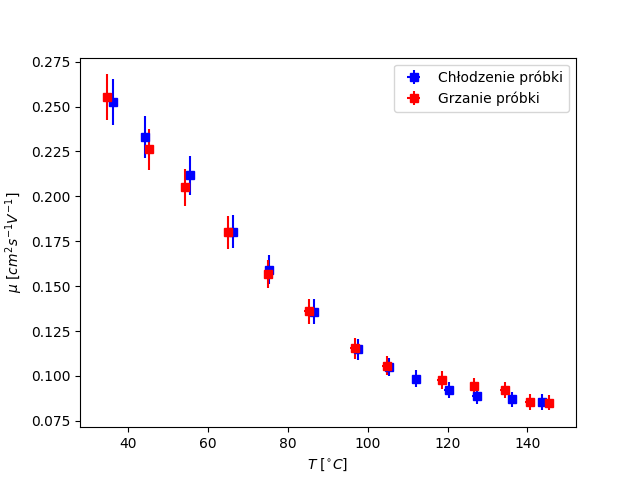
\includegraphics[scale=0.5]{temp_mobility}
    \caption{Zależność mobilności nośników w badanej próbce od temperatury.}
    \label{fig:temp_mobility}
\end{figure}

\begin{figure}[H]
    \centering
    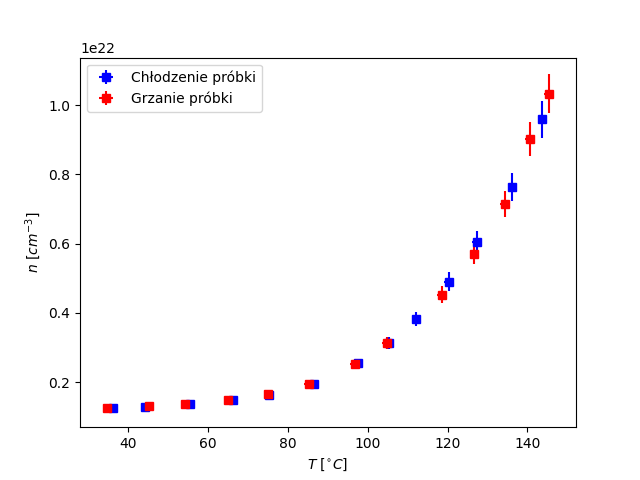
\includegraphics[scale=0.5]{temp_concentration}
    \caption{Zależność koncentracji (gęstości) nośników w badanej próbce od temperatury.}
    \label{fig:temp_concentration}
\end{figure}

Widzimy, że wraz ze wzrostem temperatury koncentracja nośników stale rośnie, a mobilność maleje. Tłumaczy to spadek oporu próbki przy podwyższaniu temperatury, ponieważ szybko rosnąca liczba nośników przeważa nad zmniejszaniem się ich ruchliwości (spowodowanym wzrostem rozpraszania na drganiach sieci krystalicznej).

\subsection{Wyznaczanie energii aktywacji}
W zakresie wysokich temperatur (ponad $100$--$110\,^\circ\mathrm{C}$ w naszych pomiarach) możemy sprawdzić, czy obowiązuje wzór \eqref{eq:high_temp}. Przewodność $\sigma$ wyrażamy przez prawo Ohma:
\[
    \sigma \;=\; \frac{l\,I}{S\,U_P},
\]
zaś temperaturę $T\,[\mathrm{K}]$ otrzymujemy z przeliczenia $T_K = T_C + 273{,}15$ \cite{kelvin}.  
Zależność zapisujemy jako:
\[
    \log(\sigma) \;=\; \log(\sigma_0)\;-\;\frac{E_{A_s}}{2\,k}\,\frac{1}{T}.
\]

\begin{figure}[H]
  \centering
  \begin{subfigure}[b]{0.45\textwidth}
    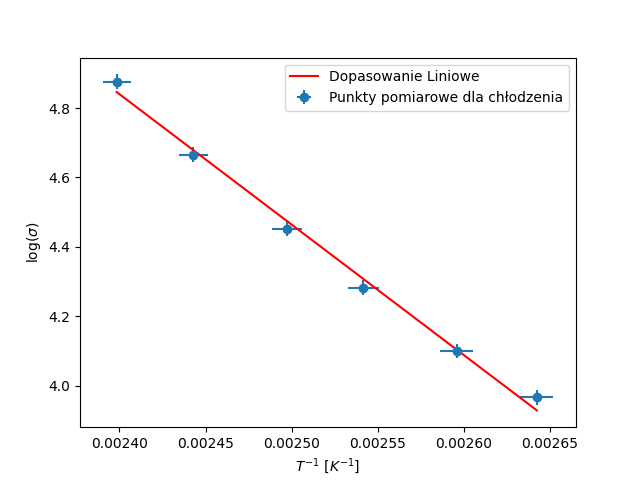
\includegraphics[width=\textwidth]{temp_cooling_fit}
    \caption{Dopasowanie dla ostatnich 6 pomiarów przy chłodzeniu ($T>105{,}3\,^\circ\mathrm{C}$).}
    \label{fig:temp_cooling_fit}
  \end{subfigure}
  \hfill
  \begin{subfigure}[b]{0.45\textwidth}
    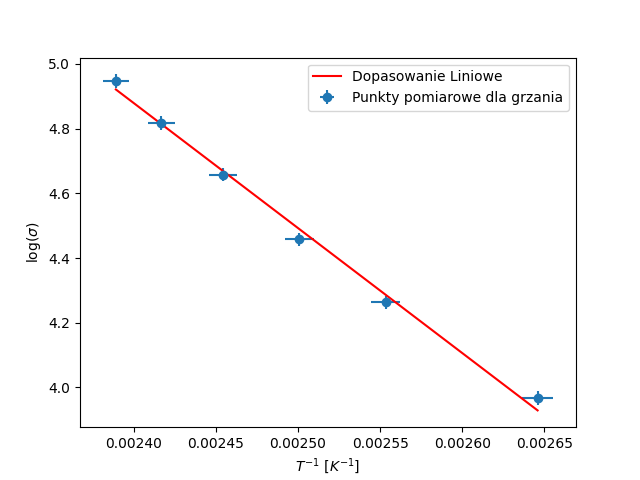
\includegraphics[width=\textwidth]{temp_heating_fit}
    \caption{Dopasowanie dla pierwszych 6 pomiarów przy ogrzewaniu ($T>104{,}8\,^\circ\mathrm{C}$).}
    \label{fig:temp_heating_fit}
  \end{subfigure}
  \caption{Dopasowanie liniowe (wykres $\log(\sigma)$ od $1/T$) w zakresach wysokich temperatur.}
  \label{fig:temp_fits}
\end{figure}

Dopasowanie liniowe (rys.~\ref{fig:temp_fits}) daje dla chłodzenia:
\begin{equation}
    \frac{E_{A_s,c}}{2\,k} = 3760\,^\circ\mathrm{C}, \quad u\!\bigl(\tfrac{E_{A_s,c}}{2\,k}\bigr) = 150\,^\circ\mathrm{C},
    \label{eq:temp_cooling_fit}
\end{equation}
zaś dla ogrzewania:
\begin{equation}
    \frac{E_{A_s,h}}{2\,k} = 3870\,^\circ\mathrm{C}, \quad u\!\bigl(\tfrac{E_{A_s,h}}{2\,k}\bigr) = 150\,^\circ\mathrm{C}.
    \label{eq:temp_heating_fit}
\end{equation}
Różnice wynikają z niedoskonałej stabilizacji temperaturowej i niejednakowego tempa nagrzewania/chłodzenia. Ostateczną wartość wyznaczamy ponownie przez średnią ważoną:
\begin{equation}
    \frac{E_{A_s}}{2\,k} = 3810\,^\circ\mathrm{C} \;\pm\; 110\,^\circ\mathrm{C}.
    \label{eq:final_cof}
\end{equation}
Korzystając z $k=1{,}380\,649\times 10^{-23}\,\mathrm{J\,K}^{-1}$ \cite{boltzman}, obliczamy:
\[
    E_{A_s} = 0{,}658\,\mathrm{eV}, 
    \quad 
    u(E_{A_s}) = 0{,}018\,\mathrm{eV}.
\]
Otrzymana wartość mieści się w przedziale przerwy energetycznej przewidywanym w literaturze \cite{band_gap}.

\newpage
\section{Podsumowanie}
W przedstawionym eksperymencie rozpoczęliśmy od wyznaczenia przewodności próbki Ge w temperaturze pokojowej, dopasowując linię do zależności napięcia od natężenia (tabela \ref{tab:ohm_measurements}), a następnie korzystając z wymiarów próbki oraz wzoru \eqref{eq:ohm_law}. Uzyskana wartość to $\sigma = 56{,}10 \pm 0{,}05\,\Omega^{-1}\mathrm{m}^{-1}$.

W celu wyznaczenia stałej Halla mierzylismy napięcie Halla dla czterech konfiguracji przy stałym natężeniu (tabela \ref{tab:const_current_measurements}) i stałym polu magnetycznym (tabela \ref{tab:const_magnetic_field_measurements}). Dopasowaliśmy zależność do wzoru \eqref{eq:hall_voltage} (rys.~\ref{fig:const_current_measuremnts}, \ref{fig:const_field_measuremnts}), a finalną wartość uzyskaliśmy poprzez średnią ważoną, otrzymując $R_H = (5{,}208 \pm 0{,}006)\times 10^{-3}\,\mathrm{m}^3\mathrm{C}^{-1}$. Znaki napięć w konfiguracji układu pomiarowego wskazują, że próbka Ge ma dodatnie nośniki (typ \emph{p}). 

Następnie, korzystając ze wzorów \eqref{eq:ohm_law} i \eqref{eq:hall_const}, wyznaczyliśmy ruchliwość nośników: $\mu = 2922 \pm 4\,\mathrm{cm}^2\mathrm{s}^{-1}\mathrm{V}^{-1}$ oraz koncentrację ładunków $n = (1{,}1985 \pm 0{,}0013)\times 10^{15}\,\mathrm{cm}^{-3}$.

W ostatniej części doświadczenia zbadaliśmy zależność napięcia na próbce oraz napięcia Halla od temperatury zarówno przy ogrzewaniu (tabela \ref{tab:heating_measurements}), jak i przy chłodzeniu (tabela \ref{tab:cooling_measurements}). Wykazaliśmy, że koncentracja nośników wzrasta wraz z temperaturą (rys.~\ref{fig:temp_concentration}), natomiast ruchliwość spada (rys.~\ref{fig:temp_mobility}). Końcowo, w zakresie wyższych temperatur dopasowaliśmy obserwowaną zależność do wzoru \eqref{eq:high_temp}, uzyskując wartość energii aktywacji nośników samoistnych $E_{A_s} = 0{,}658 \pm 0{,}018\,\mathrm{eV}$.  

Otrzymane wartości możemy porównać z typowymi danymi dla niemodyfikowanego Ge \cite{band_gap}. Zauważamy, że wyznaczony przez nas wynik dla przerwy energetycznej $E_{A_s}$ mieści się w granicach naszej niepewności wartości literaturowych. Natomiast uzyskana koncentracja ładunków okazuje się o kilka rzędów wielkości większa niż spodziewana dla niedomieszkowanego Ge, lecz jest to zrozumiałe, ponieważ wprowadzenie dodatkowych atomów domieszkowania generuje znaczący wzrost liczby nośników.
Jednocześnie wartość mobilności nośników dobrze koresponduje z danymi z \cite{electric_ge}, co wskazuje podobny rząd wielkości. Należy jednak pamiętać, że bezpośrednie porównywanie rezultatów z \cite{band_gap} i \cite{electric_ge} może być obarczone niepewnością wynikającą z obecności różnej liczby defektów w badanych próbkach oraz z odmiennego stopnia ich domieszkowania.

Błędy napotkane w eksperymencie okazały się niewielkie i w większości wynikały z niedoskonałości przyrządów pomiarowych. Główną niejasność stanowiła zmiana wartości pola magnetycznego przy odwracaniu jego kierunku — można dyskutować, czy przyjęcie błędu na poziomie największego z odchyleń jest najlepszym rozwiązaniem, jednakże uznaliśmy je za najbardziej uzasadnione podczas uśredniania napięć. Ostatecznie ów błąd został zniwelowany przez dodatkowe pomiary przy stałym polu magnetycznym, które pozwoliły obniżyć niepewność wyznaczonej stałej Halla.

\newpage

\begin{thebibliography}{9}

\bibitem{skrypt}
\emph{Wyznaczanie Ruchliwości i Koncentracji Nośników w Półprzewodniku}, Uniwersytet Warszawski, Marta Borysiewicz, Aneta Drabińska.

\bibitem{diagram}
\url{https://www.kicad.org/}, KiCad.

\bibitem{multimeter_hand}
\url{https://static.eleshop.nl/mage/media/downloads/bm805_datasheet.pdf}, multimetr Brymen BM805.

\bibitem{magnetometer}
\url{https://www.manualslib.com/manual/1980910/Voltcraft-Gm-70.html?page=33#manual}, miernik pola magnetycznego Voltcraft GM-70.

\bibitem{multimeter_big}
\url{http://pracownie1.fuw.edu.pl/przyrzady/Multimetr_Rigol_DM3058_UserGuide_EN.pdf}, multimetr Rigol DM3058.

\bibitem{charge}
\url{https://physics.nist.gov/cgi-bin/cuu/Value?e}, ładunek elektronu.

\bibitem{kelvin}
\url{https://www.nist.gov/si-redefinition/kelvin-introduction}, skala Kelvina.

\bibitem{boltzman}
\url{https://nvlpubs.nist.gov/nistpubs/SpecialPublications/NIST.SP.330-2019.pdf}, stała Boltzmanna.

\bibitem{band_gap}
\url{https://www.ioffe.ru/SVA/NSM/Semicond/Ge/bandstr.html}, Germanium Band structure and carrier concentration.

\bibitem{electric_ge}
\url{https://www.ioffe.ru/SVA/NSM/Semicond/Ge/electric.html}, Germanium Electrical properties.


\end{thebibliography}

\end{document}
